\documentclass{article}
\usepackage{graphicx}
\usepackage{amsmath} % For math formatting


\begin{document}

\title{Fall-2023 5304 LecN Notes}
\author{Wan}
\date{\today}
\maketitle



\section{Inner Products}
\subsection{Definition of Inner Products}
Notes: The notation is important and useful.\\
\\
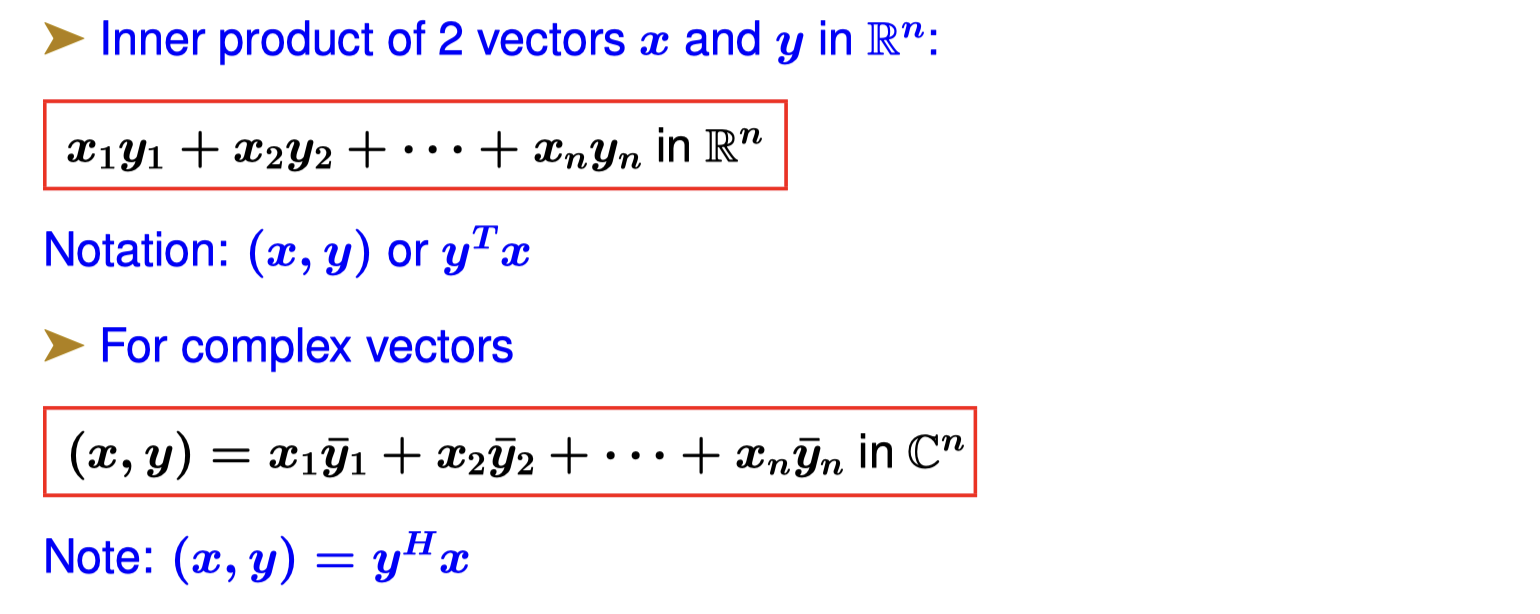
\includegraphics[width=1\linewidth]{lec2-3.png}

\subsection{Properties of inner products}
\textbf{4 operation Properties}\\
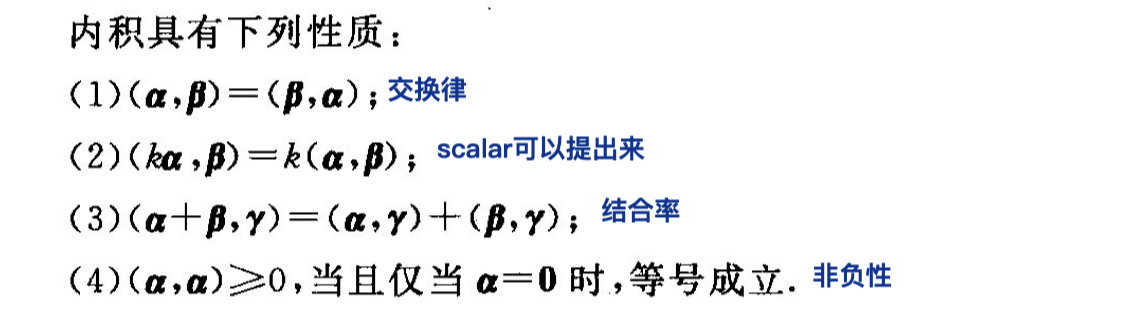
\includegraphics[width=1\linewidth]{lec2-2.png}
\\
\noindent
\textbf{1 useful property for proving}\\
\includegraphics[width=1\linewidth]{lec2-4}

\pagebreak
\section{Eigenvalues and Eigencevectors}
\subsection*{Properties of eigenvalues}
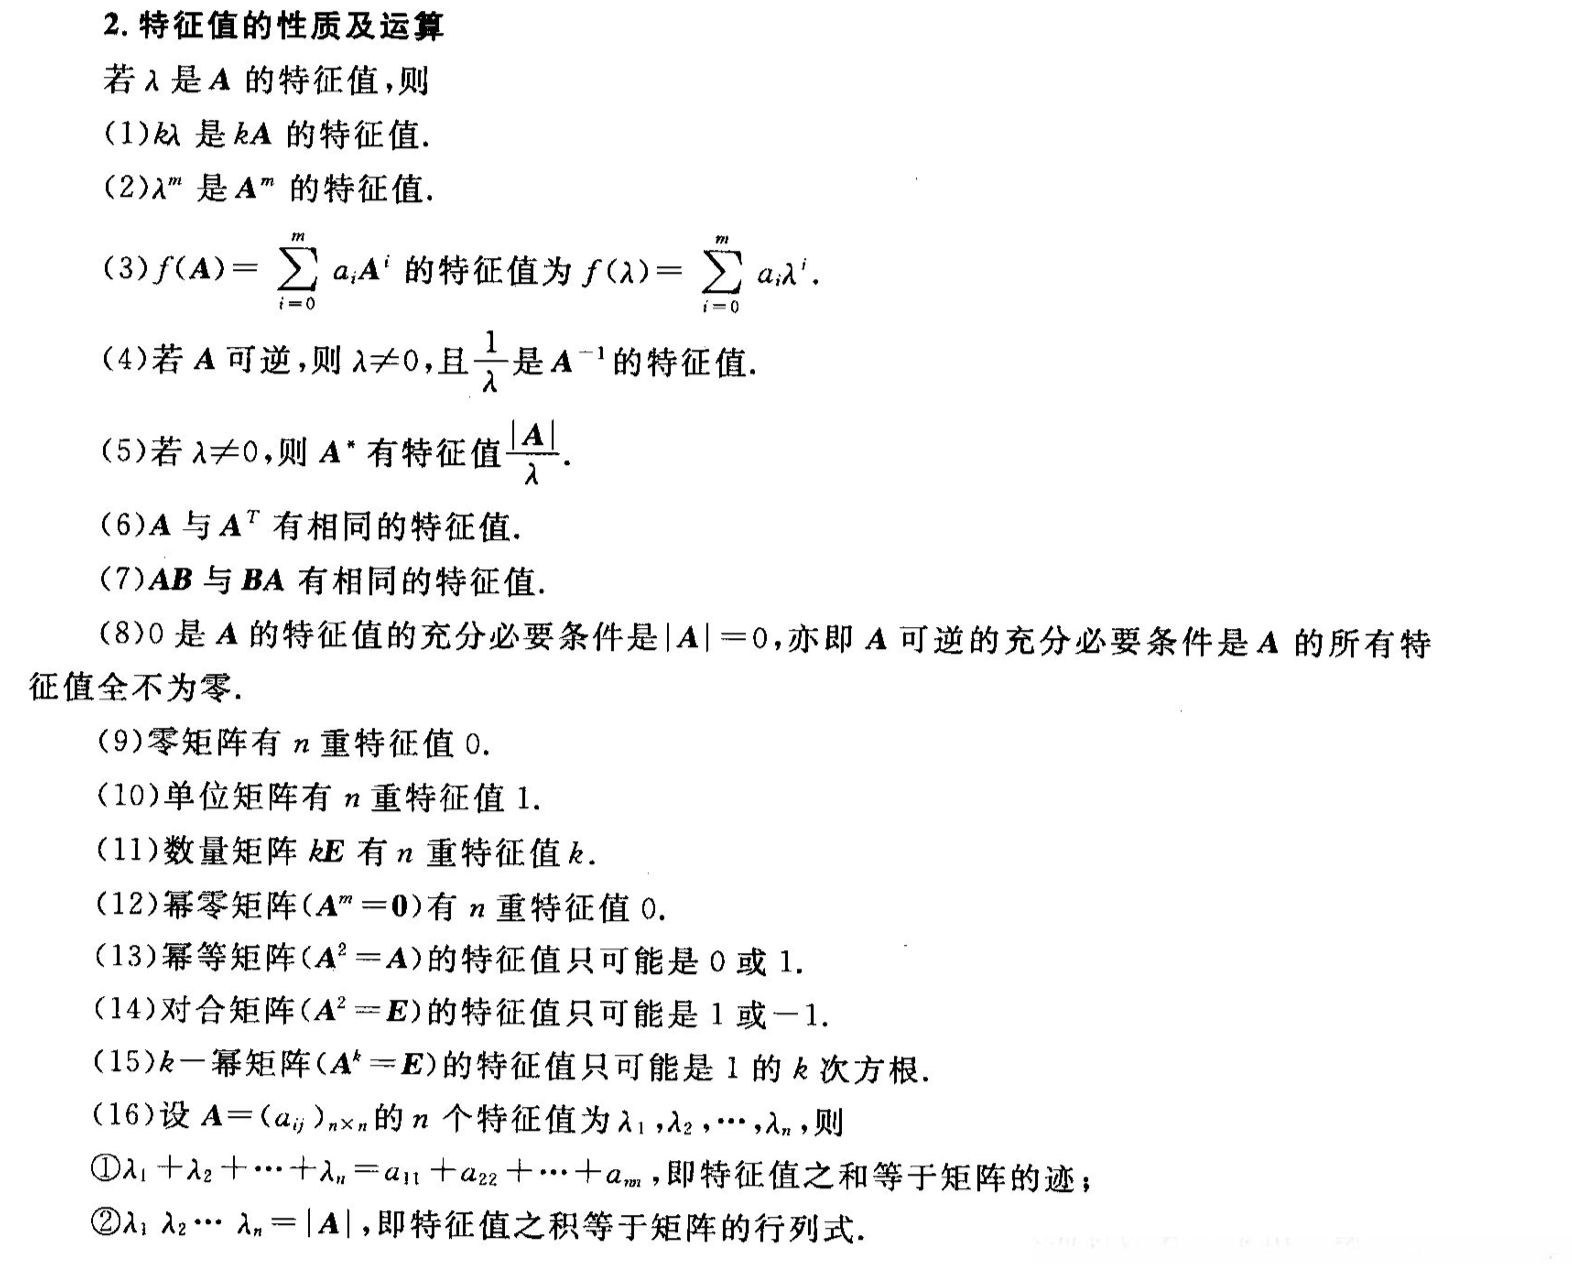
\includegraphics[width=1.5\linewidth]{lec2-1.png}

\end{document}